\section{Proposed Method}

The methodology in this to first address the \gls{MVP}, and state the  
specifications for a \gls{MVP}, see Section \ref{sec:mvs}. From there, features 
will then be added 
according to a feature list, see Section \ref{sec:features}.

\subsection{Minimum viable solution}\label{sec:mvs}

Initially, the project to aims to address the mapping phase, and if time allows 
implement a localization module as well. Since the idea is that the data will 
be ``crowd sourced'' the sensors cannot be expected to be high cost, therefore 
\gls{LIDAR} measurements are not initially considered. The types of sensor that 
first will be investigated are radio measurements, \gls{GNSS}, inertial 
navigation, and camera sensors.

Due to the separation of landmarks in radio and camera measurements, these two 
systems can provide an independent estimate of the dynamical states, $x_{1:T}$ 
and the separate landmarks $m_{r,1:T}$ for radio and $m_{v,1:T}$ for the 
camera. 

\subsection{Sensor Fusion}

Describe the sensor fusion algorithm here, EKF with information filter?

\subsection{Motion model}

As a motion model for dynamics of the vehicle, we will use the bicycle model 
adapted for a 
car.
The parameters are shown in figure \ref{fig:motion_model}. The state space 
model is defined as

\begin{equation}
 \begin{array}[b]{r}
  \dot{x}  = v \cos \theta \\
  \dot{y}  = v \sin \theta \\
  \dot{\theta}  = \frac{v}{L} \tan{\phi}
 \end{array}
\end{equation}

where $v$ is speed of the car and $\phi$ is the steering angle. 
These can be observed using an \gls{IMU} and/or estimates from the onboard car 
sensors. This provides a model for $f_k$ in Equations \eqref{eq:slam_problem}.


\begin{figure}
\centering
\label{fig:motion_model}
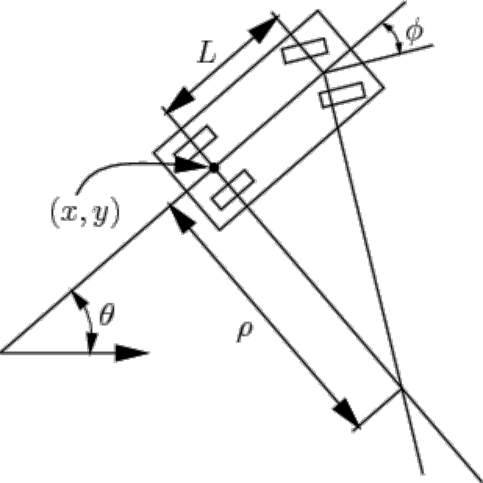
\includegraphics[width=0.3\textwidth]{figures/bicycle_model.pdf}
\caption{Bicycle motion model adapted for car}
\end{figure}


\subsection{Radio Measurements}\label{sec:radio_measurements}

The radio based localization could be summarized as three steps:

\begin{itemize}
\item Radio channel data collection. There are two options: 
  \begin{itemize}
  \item To use channel sounder and antenna arrays (with 32 antenna elements) on both base station and user sides to collect channel information with respect to angles and distances.
  \item To use a USRP with \gls{LTE} framework and switching antenna array to 
  receive commercial LTE signals from base stations.
  \end{itemize}
High spatial sampling rate of the radio channel is required, typically a few samples per wavelength movement. 
\item Radio channel parameter estimation. To use the \gls{EKF} or the 
space-alternating generalized expectation-maximization (SAGE) based estimator 
to extract geometrical information of the environment, i.e., propagation path 
parameters, for example the azimuth/elevation angle of arrival, propagation 
distance, etc. 
\item Radio based SLAM. 
\end{itemize}

The radio channel measurement will be performed locally in Lund. For sensor fusion in the late phase of this project, the measurement with different sensors will be performed simultaneously. 
\begin{itemize}
\item Scenario: daytime and outdoor; a static base station and a moving vehicle, and multiple antenna system is available on both sides. 
\item Equipment: a vehicle (or a manually moved trolley) will be used to accommodate antennas arrays, channel sounder, USRP, cameras, etc.
\item Synchronization between different sensors: different sensors will be triggered with the same TTL signal.
\item Ground truth: a camera based positioning system or a highly accurate GPS system will be used to generate ground truth for performance evaluation.     
\end{itemize}


\subsection{Features include after MVP}\label{sec:features}

Listed below are features are considered ``good to have'' but not
necessary:

\begin{itemize}
\item Radio localization  (Xuhong  Junshi)
\item Updating map:
  \begin{itemize}
  \item Update the map dynamically over time.
  \item Multiple data-sets from the same area.
  \end{itemize}
\item Large scale mapping (country size)
\item How to extract persistent features in the environment, that does
  not change over time:
  \begin{itemize}
  \item  Semantic segmentation (labelling of objects, not only ORB
    features), lanes will give lateral information, emergency doors
    will give information in the tunnel, stop signs will give
    longitudinal location
  \end{itemize}
\item Feature extractor for lanes.
\item Feature extractor for signs.
\item Handle sensor failures.
\item Include calibration parameters of the sensors in the offline processing.
\item Be able to handle different types of sensors, such as different camera types, e.g. normal lens, fish lens, HD camera.
\end{itemize}

\subsection{Sparse visual odometry}

 Sparse bundle adjustment is performed for the localization using stereo cameras. For both left and right images, ORB features are extracted at required time stamps. k-Nearest Neighbor(k-NN) matching is performed to find correspondence for static and temporal stereo. As the feature points are represented using homogeneous coordinates, static stereo is used for estimating the scale of these coordinates. After the scales are obtained, the feature points can be projected into 3D space in its local camera frame. The sparse bundle adjustment can be then performed by using temporal matched features. More specifically, the following residual is minimized to estimate the current camera pose:

	\begin{equation} \label{eq:pnp}
	E (\bm{\xi}) = \sum_i r_i(\bm{\xi}) = \sum_i ( \bm{x_i} - \pi^{-1}( \mathbf{R} \mathbf{\cdot} \pi(\bm{y_i}) + \mathbf{t}))^2
	\end{equation}
 where $\bm{\xi}$ is 6DOF parameters to be estimated and it can be represented by a rotation $\mathbf{R}$ and translation $\mathbf{t}$. $\bm{x_i}$ and $\bm{y_i}$ are matched feature pairs. $\pi$ is the warping function using camera intrinsic. 
 

\subsection{Feature extraction camera}

The landmarks extracted from the camera can be done using semantic
segmentation on the data-set \cite{Brostow:2009:SOC:1464534.1465403}.

Tutorial is found here:
\url{https://se.mathworks.com/help/vision/examples/semantic-segmentation-using-deep-learning.html}

From the segmented images, it is possible to get an \gls{AOA}
measurement. From the image, the center of gravity can be computed,
and can be compared with the field of view of the sensing camera.



\subsection{Performance assessment}

In order to assess the performance of the off-line \gls{SLAM}
algorithm, it is possible to perform cross-validation.

\subsection{Research arenas (WARA-CAT)}


The requirements on WARA-CAT are:
\begin{itemize}
  \item Test environment for data collection using the defined sensor in
    \ref{sec:sensor-setup}
\item Ground truth of the vehicle for evaluation of algorithms.
\end{itemize}


%%% Local Variables:
%%% mode: latex
%%% TeX-master: "main"
%%% End:
